\documentclass[11pt]{article}

\usepackage[letterpaper,margin=0.88in]{geometry}
\usepackage[T1]{fontenc}
\usepackage{lmodern}
\usepackage{microtype}
\usepackage{amsmath,amssymb,amsthm,mathtools,bm}
\usepackage{booktabs,array,longtable,tabularx}
\usepackage{enumitem}
\usepackage{tikz}
\usetikzlibrary{arrows.meta,calc,decorations.pathreplacing,positioning,patterns,shapes.geometric,fit,backgrounds}
\usepackage{pgfplots}
\pgfplotsset{compat=1.18}
\usepgfplotslibrary{fillbetween}
\usepackage{subcaption}
\usepackage{natbib}
\usepackage{hyperref}
\usepackage[nameinlink,capitalise,noabbrev]{cleveref}
\usepackage{xcolor}
\usepackage{siunitx}
\usepackage{fancyhdr}
\usepackage{titlesec}

\definecolor{paperblue}{RGB}{30,76,120}
\definecolor{paperred}{RGB}{150,48,42}
\definecolor{papergreen}{RGB}{46,112,75}
\definecolor{papergray}{RGB}{92,98,105}

\hypersetup{
  colorlinks=true,
  linkcolor=paperblue,
  citecolor=paperblue,
  urlcolor=paperblue,
  pdftitle={Complete Mechanics and Risk-Optimal Control of the Shoot-the-Moon Two-Rail Ball Game},
  pdfauthor={Jude Gomila}
}

\pagestyle{fancy}
\fancyhf{}
\fancyhead[L]{\small J. Gomila}
\fancyhead[R]{\small Complete Mechanics of the Two-Rail Ball Game}
\fancyfoot[C]{\thepage}
\renewcommand{\headrulewidth}{0.3pt}
\setlength{\headheight}{14pt}

\titleformat{\section}{\large\bfseries}{\thesection}{0.65em}{}
\titleformat{\subsection}{\normalsize\bfseries}{\thesubsection}{0.65em}{}
\numberwithin{equation}{section}

\newtheorem{proposition}{Proposition}[section]
\newtheorem{theorem}[proposition]{Theorem}
\newtheorem{lemma}[proposition]{Lemma}
\newtheorem{corollary}[proposition]{Corollary}
\newtheorem{conjecture}[proposition]{Conjecture}
\crefname{conjecture}{conjecture}{conjectures}
\Crefname{conjecture}{Conjecture}{Conjectures}
\theoremstyle{definition}
\newtheorem{definition}[proposition]{Definition}
\newtheorem{assumption}[proposition]{Assumption}
\theoremstyle{remark}
\newtheorem{remark}[proposition]{Remark}

\newcommand{\R}{\mathbb{R}}
\newcommand{\dd}{\,\mathrm{d}}
\newcommand{\pd}{\partial}
\newcommand{\sgn}{\operatorname{sgn}}
\newcommand{\erf}{\operatorname{erf}}
\newcommand{\safe}{\mathcal{S}}
\newcommand{\target}{\mathcal{T}}
\newcommand{\controls}{\mathcal{U}}
\newcommand{\K}{\mathcal{K}}
\newcommand{\E}{\mathbb{E}}
\newcommand{\Prob}{\mathbb{P}}

\title{\textbf{Complete Mechanics and Risk-Optimal Control of the Shoot-the-Moon Two-Rail Ball Game}\\[0.35em]
\large Rigid-body foundations, independently rotating rods, compliance, hybrid release, and maximum-score play}
\author{Jude Gomila}
\date{August 2026}

\begin{document}
\maketitle

\begin{abstract}
A steel ball supported by two player-controlled rods forms a compact but unusually rich mechanical system.  The rods rise along the board, while increasing their separation lowers the ball relative to the rod centers; this geometric competition permits apparent uphill motion.  Peng Xu, Richard Groff, and Timothy Burg established the rigid-body kinematics and nonlinear, underactuated, nonholonomic dynamics of the Shoot-the-Moon apparatus and demonstrated model-based position control in simulation and experiment.  The present paper retains that rigid foundation while developing a standalone mechanics and optimal-play treatment that includes rolling resistance, traction limits, independent rod attitude, approximately five-degree axial rotation of each rod, slight bending and torsion, contact loss, free flight, scoring geometry, target-specific viability, and risk-sensitive control.

For symmetric circular rails, the normalized separation $\eta=d/[2(R+r)]$ and support margin $\delta=\sqrt{1-\eta^2}$ give an exact local rolling radius $R_{\mathrm{eff}}=R\delta$ and effective translational mass $M=m(1+\kappa/\delta^2)$.  A critical opening condition and terminal rotational regularization follow.  Independent axial rod angles $\phi_\pm$ enter through the moving-surface contact velocity.  In the locally parallel circular-rail limit, common twist sets ball spin about the rail direction, while differential twist is kinematically conjugate to cross-sectional center motion; incompatible twist produces microslip.  Divergence, skew, noncircularity, and elastic torsion create additional coupling into longitudinal propulsion and braking.  A beam-compliance closure has an explicit fold at $\delta_*=\Lambda^{1/3}$, and the terminal drop is formulated as a hybrid transition.  Under Gaussian release-timing uncertainty, hit probability decreases strictly with speed.  The observed maximum-score strategy is therefore a boundary-riding risk problem.  Pontryagin's principle explains high-authority compound pulses, while the claim that exactly one dominant intermediate separation--twist pulse is globally optimal is stated as a falsifiable conjecture.
\end{abstract}

\noindent\textbf{Keywords.} Shoot-the-Moon; rolling sphere; independently rotating rails; nonholonomic contact; compliant rods; hybrid mechanics; viability kernel; risk-sensitive optimal control; bang-bang control.

\medskip
\noindent\textbf{MSC 2020.} 70E18, 70F25, 74H15, 49J15, 93C10.

\section{Introduction}

The apparatus consists of a rigid ball supported by two slender cylindrical rods.  The rods are close together near a hinge and are manipulated independently at their opposite ends.  Their centerlines can open and close, acquire small individual yaw and pitch differences, and rotate slightly about their own axes.  Inspection of the game mechanism suggests an axial rotational excursion of order $5^\circ$ per rod; throughout this paper this is treated as the nominal bound
\begin{equation}
  |\phi_i|\lesssim\phi_{\max},
  \qquad
  \phi_{\max}=5^\circ\approx 0.0873\ \mathrm{rad},
  \label{eq:nominaltwist}
\end{equation}
subject to direct measurement on the particular apparatus.

The mean rail direction is inclined upward, yet opening the rods lowers the ball center enough to produce motion toward the high end.  The player then releases the ball through one of several scoring apertures.  A maximum-score run must combine sufficient travel, retained contact, and precise terminal timing.  The central playing observation is a risk paradox: the terminal target appears to favor a strong pulse in an intermediate region and a passage at nearly the greatest controllable speed.  That strategy simultaneously narrows the timing window and leaves little recovery authority.

The rigid-body foundation is due to Xu, Groff, and Burg.  Their conference paper, thesis, and journal article derive the kinematics and equations of motion, identify the system as underactuated, nonlinear, and nonholonomic, design linearized and nonlinear position controllers, and validate the nonlinear controller on an automated physical apparatus \citep{Xu2010,Xu2011,Xu2012}.  Xu's thesis also explicitly identifies the rapid ``shoot'' phenomenon as an interaction between ball rotation and translation and demonstrates the nonholonomic relation between linear and angular position.  Accordingly, this paper does not claim the first dynamics or control model of the game.

The purpose here is broader and different: to give a standalone end-to-end mechanics guide and formulate the score-optimal human-playing problem.  The paper re-derives the symmetric geometry needed for self-containment, treats Xu's rigid model as the limiting foundation, and adds:
\begin{enumerate}[label=(\roman*),leftmargin=2.2em]
  \item independent centerline yaw and pitch of the two rods;
  \item independent axial rod rotation and moving-surface rolling constraints;
  \item common/differential twist modes, twist-induced spin, and slip compatibility;
  \item geometry-dependent effective inertia, resistance, traction, and load guards;
  \item bending and torsional compliance, including an explicit support-branch fold;
  \item hybrid transitions among rolling, slip, one-contact motion, free flight, and impact;
  \item target-specific viability, release uncertainty, and score-risk optimization;
  \item a precise, testable compound-pulse conjecture.
\end{enumerate}

\begin{figure}[t]
\centering
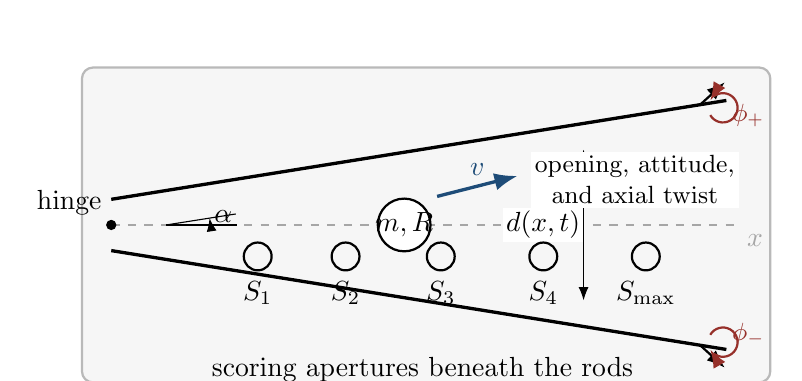
\begin{tikzpicture}[scale=0.93,>=Latex]
  \fill[gray!7,rounded corners=4pt] (-0.4,-2.15) rectangle (9.0,2.15);
  \draw[gray!55,thick,rounded corners=4pt] (-0.4,-2.15) rectangle (9.0,2.15);
  \draw[dashed,gray!70] (0,0) -- (8.55,0) node[below right] {$x$};
  \draw[very thick] (0,0.35) -- (8.4,1.70);
  \draw[very thick] (0,-0.35) -- (8.4,-1.70);
  \fill (0,0) circle (2pt) node[above left] {hinge};
  \draw[<->] (6.45,-1.03) -- (6.45,1.03) node[midway,left,fill=white,inner sep=1pt] {$d(x,t)$};
  \draw[fill=white,thick] (4.0,0) circle (0.36) node {$m,R$};
  \draw[->,very thick,paperblue] (4.45,0.39) -- (5.55,0.67) node[midway,above] {$v$};
  \draw[->,thick] (8.05,1.65) -- (8.38,1.95);
  \draw[->,thick] (8.05,-1.65) -- (8.38,-1.95);
  \draw[->,paperred,thick] (8.18,1.50) arc[start angle=210,end angle=510,radius=0.20];
  \draw[->,paperred,thick] (8.18,-1.50) arc[start angle=150,end angle=-150,radius=0.20];
  \node[paperred,font=\small] at (8.70,1.50) {$\phi_+$};
  \node[paperred,font=\small] at (8.70,-1.50) {$\phi_-$};
  \node[align=center,font=\small,fill=white,inner sep=1.5pt] at (7.15,0.62) {opening, attitude,\\and axial twist};
  \draw (0.75,0) -- (1.72,0);
  \draw (0.75,0) -- (1.70,0.15);
  \draw[->] (1.35,0) arc[start angle=0,end angle=9,radius=0.60];
  \node at (1.53,0.12) {$\alpha$};
  \foreach \xx/\lab in {2.0/$S_1$,3.2/$S_2$,4.5/$S_3$,5.9/$S_4$,7.3/$S_{\max}$}{
    \draw[thick] (\xx,-0.43) circle (0.19);
    \node[below] at (\xx,-0.64) {\lab};
  }
  \node[below,align=center] at (4.25,-1.68) {scoring apertures beneath the rods};
\end{tikzpicture}
\caption{Top-view idealization.  The included opening angle is $2\alpha$, while $\phi_\pm$ denote independent axial rotations of the rods.  The complete apparatus also permits small individual centerline attitude changes.  A real machine should replace the straight-rail law by measured centerlines and handle maps.}
\label{fig:overview}
\end{figure}


\section{Rigid-body foundation and attribution}
\label{sec:xufoundation}

The present paper is designed to be readable without consulting earlier work, but the provenance of the rigid-body results must be explicit.  Xu and coauthors supplied the first detailed mechanics and model-based control treatment located in the literature reviewed for this paper.  The thesis record states that Xu developed the kinematics, derived the equations by both Lagrangian and Newtonian methods, identified underactuated, nonlinear, nonholonomic dynamics, designed two position controllers, built an automated platform, compared experiment with simulation, and demonstrated the translation--rotation constraint \citep{Xu2011}.  The conference and journal versions report the same rigid-body program in condensed form \citep{Xu2010,Xu2012}.

\begin{table}[h]
\centering
\caption{Relationship between the Xu--Groff--Burg foundation and the present extension.}
\label{tab:provenance}
\begin{tabularx}{\linewidth}{@{}p{0.31\linewidth}X@{}}
\toprule
\textbf{Established by Xu and coauthors} & \textbf{Use and extension in this paper} \\
\midrule
Kinematic description and nonlinear rigid equations & Retained as the rigid limiting system; a self-contained symmetric reduction is re-derived for analysis. \\
Underactuated and nonholonomic structure & Used explicitly in the rolling constraints, effective inertia, and optimal-control formulation. \\
Linearized position regulation & Recognized as the local set-point-control solution; not presented here as a new result. \\
Nonlinear position tracking with feedforward/PD structure & Recognized as the prior model-based tracking result and experimental baseline. \\
Simulation and automated physical validation & Treated as evidence for the fidelity of the rigid foundation. \\
Rotation--translation ``shoot'' interaction & Extended to moving rod surfaces, independently commanded axial twist, compliance, slip, and score-optimal compound pulses. \\
\bottomrule
\end{tabularx}
\end{table}

The new questions are not whether the ball can be regulated to a position, but which states remain recoverable for a scoring target, how independent rod twist changes contact work, and which admissible vector control maximizes score under failure risk.

\section{Geometry of two-rail support}

\subsection{Coordinates and assumptions}

Let $x\in[0,L]$ be distance along the mean rail direction, positive uphill.  The ball has mass $m$, radius $R$, and central moment of inertia
\begin{equation}
  I=\kappa mR^2,
  \qquad \kappa=\frac25
  \quad\text{for a homogeneous solid sphere}.
  \label{eq:inertia}
\end{equation}
Each rod has nominal circular radius $r$, and $a:=R+r$.

For the complete three-dimensional geometry, represent rod $i\in\{+,-\}$ by a centerline
\begin{equation}
  \bm c_i(s,t)=\bm p_i(t)+s\bm t_i(t)+\bm w_i(s,t),
  \qquad 0\leq s\leq L,
  \label{eq:rodcenterline}
\end{equation}
where $\bm p_i$ is a reference point, $\bm t_i$ is a unit centerline tangent, and $\bm w_i$ is elastic displacement.  Using signed yaw $\gamma_i$ and pitch $\beta_i$,
\begin{equation}
  \bm t_i=
  \begin{bmatrix}
  \cos\beta_i\cos\gamma_i &
  \cos\beta_i\sin\gamma_i &
  \sin\beta_i
  \end{bmatrix}^{T}.
  \label{eq:rodattitude}
\end{equation}
The independent axial angle $\phi_i$ rotates the material surface about $\bm t_i$.  Convenient control modes are
\begin{align}
  \alpha_o&=\frac{\gamma_+-\gamma_-}{2},
  &\alpha_s&=\frac{\gamma_++\gamma_-}{2},\\
  \beta_c&=\frac{\beta_++\beta_-}{2},
  &\beta_d&=\frac{\beta_+-\beta_-}{2},\\
  \phi_c&=\frac{\phi_++\phi_-}{2},
  &\phi_\Delta&=\frac{\phi_- -\phi_+}{2}.
  \label{eq:controlmodes}
\end{align}
Here $\alpha_o$ is symmetric opening, $\alpha_s$ is centerline skew, $\beta_c$ is common incline, $\beta_d$ is differential cross-slope, $\phi_c$ is common axial twist, and $\phi_\Delta$ is differential axial twist.

The symmetric rigid reduction used for closed-form analysis sets $\gamma_\pm=\pm\alpha$, $\beta_\pm=\beta$, $\bm w_i=0$, and initially $\phi_\pm=0$.  Its rail-center plane rises according to
\begin{equation}
  z_r(x)=z_0+x\sin\beta,
  \label{eq:railheight}
\end{equation}
and its center-to-center separation is
\begin{equation}
  d(x,t)=d_0+2x\tan\alpha(t).
  \label{eq:separation}
\end{equation}
A real apparatus should use calibrated centerlines $\bm c_i(s,u_i)$, not assume this affine law.


\begin{figure}[t]
\centering
\begin{subfigure}[t]{0.48\linewidth}
\centering
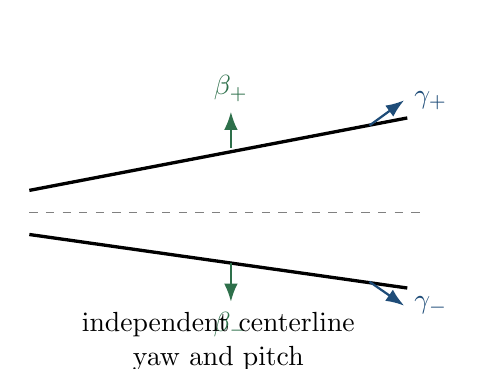
\begin{tikzpicture}[scale=0.80,>=Latex]
  \draw[dashed,gray] (0,0)--(6.3,0);
  \draw[very thick] (0,0.35)--(6.0,1.50);
  \draw[very thick] (0,-0.35)--(6.0,-1.20);
  \draw[->,paperblue,thick] (5.4,1.38)--(5.95,1.78) node[right] {$\gamma_+$};
  \draw[->,paperblue,thick] (5.4,-1.10)--(5.95,-1.48) node[right] {$\gamma_-$};
  \draw[->,papergreen,thick] (3.2,1.03)--(3.2,1.60) node[above] {$\beta_+$};
  \draw[->,papergreen,thick] (3.2,-0.80)--(3.2,-1.42) node[below] {$\beta_-$};
  \node[align=center] at (3.0,-2.05) {independent centerline\\yaw and pitch};
\end{tikzpicture}
\caption{Centerline attitude controls.}
\end{subfigure}\hfill
\begin{subfigure}[t]{0.48\linewidth}
\centering
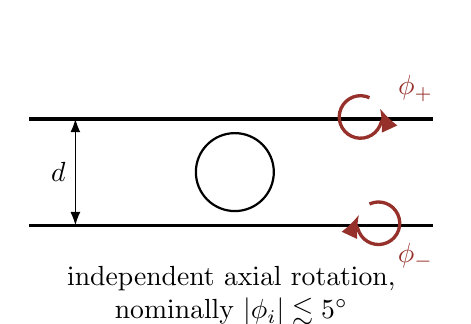
\begin{tikzpicture}[scale=0.90,>=Latex]
  \draw[very thick] (0,0.75)--(5.7,0.75);
  \draw[very thick] (0,-0.75)--(5.7,-0.75);
  \draw[fill=white,thick] (2.9,0) circle (0.55);
  \draw[->,paperred,very thick] (4.8,1.05) arc[start angle=65,end angle=385,radius=0.30];
  \draw[->,paperred,very thick] (4.8,-0.45) arc[start angle=115,end angle=-205,radius=0.30];
  \node[paperred] at (5.45,1.18) {$\phi_+$};
  \node[paperred] at (5.45,-1.18) {$\phi_-$};
  \draw[<->] (0.65,-0.75)--(0.65,0.75) node[midway,left] {$d$};
  \node[align=center] at (2.85,-1.75) {independent axial rotation,\\nominally $|\phi_i|\lesssim5^\circ$};
\end{tikzpicture}
\caption{Axial surface controls.}
\end{subfigure}
\caption{A complete handle model has more than one scalar opening coordinate.  Symmetric opening is only one mode among centerline skew, common/differential pitch, and common/differential axial rotation.}
\label{fig:sixmodes}
\end{figure}

\subsection{Cross-sectional support}

In transverse cross-section, the ball center is a distance $a$ from either rod center.  If $h$ is its height above the rod-center plane,
\begin{equation}
  \left(\frac d2\right)^2+h^2=a^2,
  \qquad
  h(d)=\sqrt{a^2-\frac{d^2}{4}}.
  \label{eq:h}
\end{equation}
Introduce the dimensionless separation and support margin
\begin{equation}
  \eta:=\frac{d}{2a},
  \qquad
  \delta:=\sqrt{1-\eta^2},
  \qquad
  h=a\delta.
  \label{eq:etadelta}
\end{equation}
The rigid geometric support limit is $\eta\uparrow1$, equivalently $\delta\downarrow0$.

\begin{proposition}[Monotone, concave support height]
For $0<d<2a$,
\begin{equation}
  h_d=-\frac{d}{4h}<0,
  \qquad
  h_{dd}=-\frac{1}{4h}-\frac{d^2}{16h^3}<0.
  \label{eq:hderivatives}
\end{equation}
Thus opening the rods lowers the ball center, and the magnitude of geometric sensitivity increases without bound as $\delta\downarrow0$.
\end{proposition}

\begin{proof}
Differentiate \cref{eq:h} once and twice with respect to $d$.
\end{proof}

\begin{figure}[t]
\centering
\begin{subfigure}[t]{0.48\linewidth}
\centering
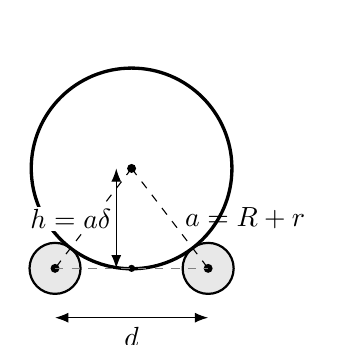
\begin{tikzpicture}[scale=1.08,>=Latex]
  \coordinate (RL) at (-0.90,0);
  \coordinate (RR) at (0.90,0);
  \coordinate (B) at (0,0);
  \coordinate (C) at (0,1.175);
  \draw[fill=gray!18,thick] (RL) circle (0.30);
  \draw[fill=gray!18,thick] (RR) circle (0.30);
  \draw[fill=white,very thick] (C) circle (1.18);
  \fill (RL) circle (1.5pt); \fill (RR) circle (1.5pt); \fill (B) circle (1.2pt); \fill (C) circle (1.5pt);
  \draw[dashed] (C) -- (RL);
  \draw[dashed] (C) -- (RR) node[midway,right=2pt] {$a=R+r$};
  \draw[dashed,gray] (RL) -- (RR);
  \draw[<->] (-0.18,0) -- (-0.18,1.175);
  \node[left,fill=white,inner sep=1pt] at (-0.20,0.58) {$h=a\delta$};
  \draw[<->] (-0.90,-0.58) -- (0.90,-0.58) node[midway,below] {$d$};
\end{tikzpicture}
\caption{Exact transverse geometry.}
\label{fig:crosssection}
\end{subfigure}\hfill
\begin{subfigure}[t]{0.49\linewidth}
\centering
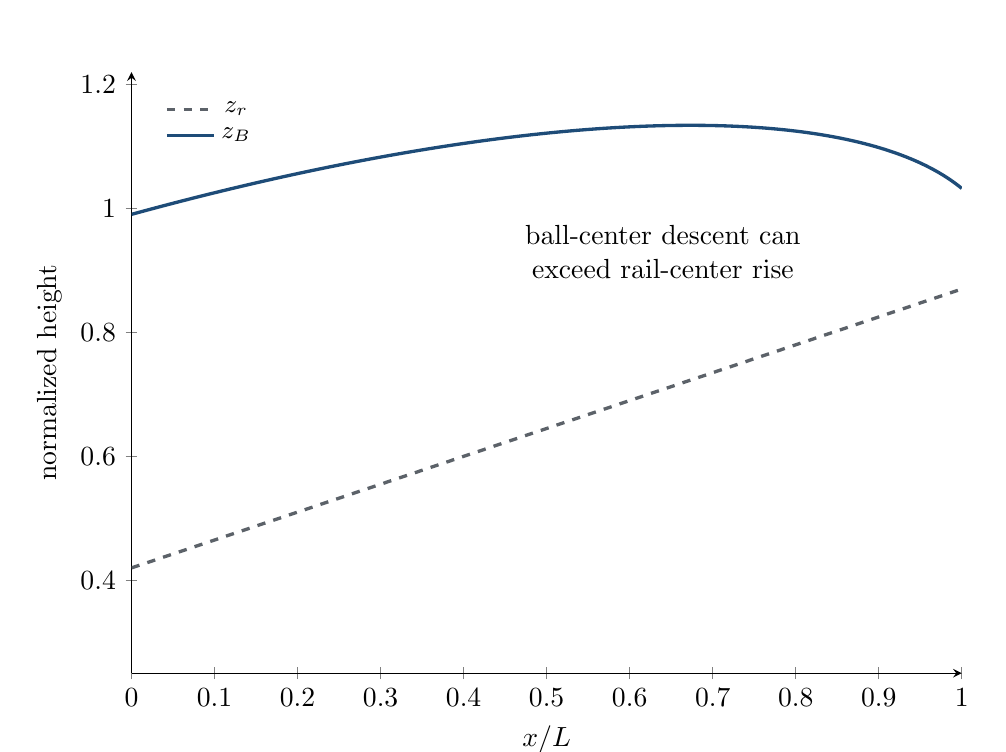
\begin{tikzpicture}
\begin{axis}[
 width=\linewidth,height=0.76\linewidth,
 axis lines=left,xlabel={$x/L$},ylabel={normalized height},
 xmin=0,xmax=1,ymin=0.25,ymax=1.22,
 legend style={draw=none,font=\small,at={(0.03,0.97)},anchor=north west},
 samples=180,domain=0:1]
 \addplot[very thick,dashed,papergray] {0.42+0.45*x};
 \addlegendentry{$z_r$}
 \addplot[very thick,paperblue] {0.42+0.45*x+0.58*sqrt(1-(0.18+0.78*x)^2)};
 \addlegendentry{$z_B$}
 \node[align=center,fill=white,inner sep=1.2pt] at (axis cs:0.64,0.93) {ball-center descent can\\exceed rail-center rise};
\end{axis}
\end{tikzpicture}
\caption{Illustrative height decomposition.}
\label{fig:height}
\end{subfigure}
\caption{The same support margin $\delta$ controls ball height, contact orientation, rolling kinematics, and normal load.  The plotted height curves are schematic, not fitted data.}
\label{fig:geometry}
\end{figure}

The ball-center height and potential energy are
\begin{equation}
  z_B(x,\alpha)=z_0+x\sin\beta+a\delta(x,\alpha),
  \qquad
  V(x,\alpha)=mgz_B(x,\alpha).
  \label{eq:zV}
\end{equation}

\section{Exact symmetric rolling reduction}

\subsection{Contact kinematics}

Let $\bm e_x$ point along the mean rail direction, $\bm e_y$ transversely, and $\bm e_z$ normally away from the rail-center plane.  The unit normal forces on the ball are directed along
\begin{equation}
  \bm n_\pm=\mp\eta\bm e_y+\delta\bm e_z,
  \label{eq:normals}
\end{equation}
where $+$ and $-$ label the right and left rods.  The radius vectors from the ball center to the contact points are
\begin{equation}
  \bm\rho_\pm=-R\bm n_\pm.
\end{equation}
For symmetric longitudinal rolling, take $\bm\omega=\omega\bm e_y$.  On stationary rods the longitudinal no-slip condition is
\begin{equation}
  0=\bigl(v\bm e_x+\bm\omega\times\bm\rho_\pm\bigr)\cdot\bm e_x
   =v-R\delta\omega.
\end{equation}
Therefore
\begin{equation}
  v=R_{\mathrm{eff}}\omega,
  \qquad
  R_{\mathrm{eff}}=R\delta.
  \label{eq:reff}
\end{equation}

\begin{proposition}[Geometry-dependent effective mass]
Under symmetric no-slip rolling,
\begin{equation}
  T=\frac12M(x,\alpha)v^2,
  \qquad
  M(x,\alpha)=m\left(1+\frac{\kappa}{\delta(x,\alpha)^2}\right).
  \label{eq:Meff}
\end{equation}
\end{proposition}

\begin{proof}
Substitute $\omega=v/(R\delta)$ from \cref{eq:reff} into
$T=\frac12mv^2+\frac12I\omega^2$ and use \cref{eq:inertia}.
\end{proof}


\section{Independent axial rotation of the rods}
\label{sec:rodrotation}

\subsection{Moving cylindrical surfaces}

Let rod $i$ have centerline velocity $\dot{\bm c}_i$ and angular velocity
\begin{equation}
  \bm\Omega_i
  =\bm\Omega_{\mathrm{att},i}
   +\dot\phi_i\bm t_i
   +\dot\vartheta_i(s,t)\bm t_i,
  \label{eq:rodangularvelocity}
\end{equation}
where $\bm\Omega_{\mathrm{att},i}$ arises from changing centerline attitude and $\vartheta_i$ is elastic torsional twist.  For a circular rod, the material velocity at the contact point is
\begin{equation}
  \bm v_{r,i}
  =\dot{\bm c}_i
   +\bm\Omega_i\times(r\bm n_i),
  \label{eq:rodsurfacevelocity}
\end{equation}
where $\bm n_i$ points from the rod centerline toward the ball center.  The no-slip constraint is therefore
\begin{equation}
  \bm P_{T,i}
  \left(
  \dot{\bm r}_C+\bm\omega\times\bm\rho_i-\bm v_{r,i}
  \right)=\bm0.
  \label{eq:movingsurfacenoslip}
\end{equation}
A static axial angle $\phi_i$ does not change the geometry of a perfectly circular, homogeneous rod; only $\dot\phi_i$ changes surface velocity.  The angle itself becomes geometrically relevant when the rod has ovality, eccentricity, texture, wear, or a nonaxisymmetric coating.

\subsection{Common and differential twist in the local parallel limit}

In the locally parallel symmetric reduction, define
\begin{equation}
  \bm q_\pm:=\bm e_x\times\bm n_\pm
  =-\delta\bm e_y\mp\eta\bm e_z.
  \label{eq:qpm}
\end{equation}
Axial rod rotation creates the surface velocity
\begin{equation}
  \bm v^{\mathrm{tw}}_{r,\pm}
  =r\dot\phi_\pm\bm q_\pm.
  \label{eq:twistsurfacevelocity}
\end{equation}
Allow the ball center to have cross-sectional velocity
$\dot y\bm e_y+\dot z\bm e_z$.  Projection of \cref{eq:movingsurfacenoslip} onto $\bm q_\pm$ gives
\begin{align}
  -\delta\dot y-\eta\dot z-R\omega_x&=r\dot\phi_+,
  \label{eq:twistplus}\\
  -\delta\dot y+\eta\dot z-R\omega_x&=r\dot\phi_-.
  \label{eq:twistminus}
\end{align}
Define $\dot\phi_c=(\dot\phi_++\dot\phi_-)/2$ and
$\dot\phi_\Delta=(\dot\phi_- -\dot\phi_+)/2$.  Then
\begin{equation}
  R\omega_x+\delta\dot y=-r\dot\phi_c,
  \qquad
  \eta\dot z=r\dot\phi_\Delta.
  \label{eq:twistmodes}
\end{equation}

\begin{proposition}[Meaning of the two twist modes]
\label{prop:twistmodes}
For centered motion $\dot y=0$ on locally parallel circular rods, compatible no-slip motion satisfies
\begin{equation}
  \omega_x=-\frac rR\dot\phi_c,
  \qquad
  \dot z=\frac r\eta\dot\phi_\Delta.
  \label{eq:twistinterpretation}
\end{equation}
Thus common twist commands ball spin about the rail direction, while differential twist is kinematically conjugate to cross-sectional center motion.
\end{proposition}

\begin{proof}
Add and subtract \cref{eq:twistplus,eq:twistminus} and impose $\dot y=0$.
\end{proof}

Projection of the same no-slip equations along $\bm e_x$ yields
\begin{equation}
  \omega_y=\frac{v}{R\delta},
  \qquad \omega_z=0,
  \label{eq:twistlongitudinalspin}
\end{equation}
so compatible centered motion has
\begin{equation}
  \bm\omega
  =-\frac rR\dot\phi_c\bm e_x
   +\frac{v}{R\delta}\bm e_y.
  \label{eq:fullsymomega}
\end{equation}
The corresponding kinetic energy contribution is
\begin{equation}
  T
  =\frac12M(x,\alpha)v^2
   +\frac12\kappa mr^2\dot\phi_c^2.
  \label{eq:twistkineticenergy}
\end{equation}
In the ideal parallel circular limit, the two spin energies are orthogonal and do not automatically exchange.  Divergence, skew, changing contact normals, slip, or nonaxisymmetric surfaces create conversion mechanisms.

If the commanded differential twist is incompatible with the geometry-determined center velocity, define the slip residual
\begin{equation}
  s_\Delta:=r\dot\phi_\Delta-\eta\dot z_B.
  \label{eq:differentialslip}
\end{equation}
No-slip requires $s_\Delta=0$; otherwise the contact pair must accommodate the mismatch through elastic deformation, one-contact motion, or microslip.

\subsection{Divergent rods and direct longitudinal coupling}

For the full rod tangent $\bm t_i$, axial twist contributes longitudinal material velocity
\begin{equation}
  v^{\mathrm{tw}}_{x,i}
  =r\dot\phi_i
  (\bm t_i\times\bm n_i)\cdot\bm e_x.
  \label{eq:twistlongitudinalcoupling}
\end{equation}
This term vanishes in the local parallel idealization but is generally nonzero for divergent, pitched, skewed, or deformed rods.  For small angular departures it is of order $r|\dot\phi_i|\,O(|\gamma_i|+|\beta_d|+\|\bm w_{i,s}\|)$.  Independent axial rotation can therefore supply propulsion, braking, spin shaping, or intentional slip in the complete game.

\subsection{Noncircularity and angle-dependent geometry}

Let a weakly noncircular local radius be
\begin{equation}
  r_i(\chi,\phi_i)
  =r\left[1+\epsilon_i\cos k_i(\chi-\phi_i)\right],
  \qquad |\epsilon_i|\ll1.
  \label{eq:noncircularradius}
\end{equation}
The contact gap is then
\begin{equation}
  g_i
  =\|\bm r_C-\bm c_i\|-R-r_i(\chi_i,\phi_i).
  \label{eq:noncirculargap}
\end{equation}
Now $g_{i,\phi_i}\neq0$, so even a static $5^\circ$ rotation can change support height, normal load, and friction.  This effect should be measured before treating the rods as perfectly circular.

\begin{figure}[t]
\centering
\begin{subfigure}[t]{0.49\linewidth}
\centering
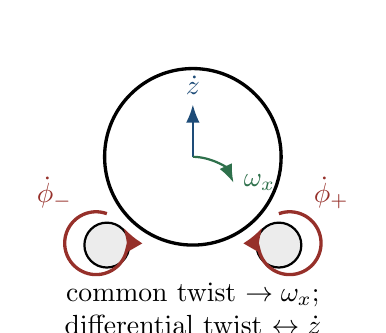
\begin{tikzpicture}[scale=0.95,>=Latex]
  \draw[fill=gray!15,thick] (-1.15,0) circle (0.30);
  \draw[fill=gray!15,thick] (1.15,0) circle (0.30);
  \draw[fill=white,very thick] (0,1.18) circle (1.18);
  \draw[->,paperred,very thick] (-1.15,0.42) arc[start angle=70,end angle=390,radius=0.42];
  \draw[->,paperred,very thick] (1.15,0.42) arc[start angle=110,end angle=-210,radius=0.42];
  \node[paperred] at (-1.85,0.70) {$\dot\phi_-$};
  \node[paperred] at (1.85,0.70) {$\dot\phi_+$};
  \draw[->,paperblue,thick] (0,1.18)--(0,1.88) node[above] {$\dot z$};
  \draw[->,papergreen,thick] (0,1.18) arc[start angle=90,end angle=25,radius=0.60] node[right] {$\omega_x$};
  \node[align=center] at (0,-0.85) {common twist $\to\omega_x$;\\differential twist $\leftrightarrow\dot z$};
\end{tikzpicture}
\caption{Cross-sectional twist modes.}
\end{subfigure}\hfill
\begin{subfigure}[t]{0.49\linewidth}
\centering
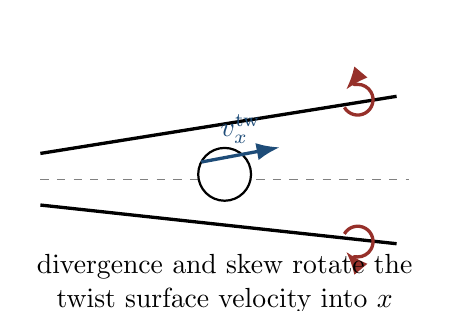
\begin{tikzpicture}[scale=0.78,>=Latex]
  \draw[dashed,gray] (0,0)--(6.0,0);
  \draw[very thick] (0,0.42)--(5.8,1.35);
  \draw[very thick] (0,-0.42)--(5.8,-1.05);
  \draw[fill=white,thick] (3.0,0.08) circle (0.43);
  \draw[->,paperred,very thick] (4.95,1.17) arc[start angle=210,end angle=500,radius=0.25];
  \draw[->,paperred,very thick] (4.95,-0.89) arc[start angle=150,end angle=-140,radius=0.25];
  \draw[->,paperblue,very thick] (2.62,0.28)--(3.90,0.52) node[midway,above] {$v^{\mathrm{tw}}_x$};
  \node[align=center] at (3.0,-1.70) {divergence and skew rotate the\\twist surface velocity into $x$};
\end{tikzpicture}
\caption{Full-geometry coupling.}
\end{subfigure}
\caption{Independent rod rotation adds genuine control channels.  The absolute angle matters only through nonaxisymmetry; the rate always matters through contact-surface velocity.}
\label{fig:rodrotation}
\end{figure}

\subsection{Reduced Lagrange equation}

For prescribed $\alpha(t)$, define
\begin{equation}
  \mathcal L(x,v;\alpha)=\frac12M(x,\alpha)v^2-V(x,\alpha).
  \label{eq:Lagrangian}
\end{equation}
Let $F_d(v,x,\alpha)$ denote the longitudinal dissipative force magnitude opposing motion.  The Euler--Lagrange equation is
\begin{equation}
  M\dot v+\frac12M_xv^2+M_\alpha\dot\alpha\,v+V_x=-F_d.
  \label{eq:reducedmotion}
\end{equation}
From \cref{eq:separation,eq:etadelta},
\begin{align}
  \eta_x&=\frac{\tan\alpha}{a},
  &\eta_\alpha&=\frac{x\sec^2\alpha}{a},\\
  \delta_x&=-\frac{\eta\tan\alpha}{a\delta},
  &\delta_\alpha&=-\frac{\eta x\sec^2\alpha}{a\delta}.
  \label{eq:deltaderivatives}
\end{align}
Consequently,
\begin{align}
  -V_x
   &=mg\left(\frac{\eta\tan\alpha}{\delta}-\sin\beta\right),
   \label{eq:drive}\\
  M_x
   &=\frac{2m\kappa\eta\tan\alpha}{a\delta^4},
  &M_\alpha
   &=\frac{2m\kappa\eta x\sec^2\alpha}{a\delta^4}.
  \label{eq:Mderivatives}
\end{align}
The first term in \cref{eq:drive} is geometry-induced uphill drive, while the second is ordinary downhill gravity.

\section{Uphill drive and terminal asymptotics}

Define the dimensionless local drive margin
\begin{equation}
  \Gamma(x,\alpha)
  :=\frac{\eta\tan\alpha}{\delta}-\sin\beta.
  \label{eq:Gamma}
\end{equation}

\begin{proposition}[Local opening threshold]
\label{prop:threshold}
At a fixed local separation $(\eta,\delta)$, with $v=0$ and negligible dissipation, the ball accelerates uphill if and only if $\Gamma>0$.  Equivalently,
\begin{equation}
  \tan\alpha>\frac{\delta\sin\beta}{\eta}
  =\frac{2h\sin\beta}{d}.
  \label{eq:criticalopening}
\end{equation}
When $d$ itself depends on $\alpha$, \cref{eq:criticalopening} is an implicit local threshold equation.
\end{proposition}

\begin{proof}
At rest the velocity-dependent terms in \cref{eq:reducedmotion} vanish.  With $F_d=0$, one has $M\dot v=-V_x=mg\Gamma$.  Since $M>0$, the sign of $\dot v$ equals the sign of $\Gamma$.
\end{proof}

A naive inspection of \cref{eq:drive} suggests an unbounded uphill force as $\delta\downarrow0$.  The rolling inertia in \cref{eq:Meff} changes that conclusion.

\begin{proposition}[Rotational regularization at zero speed]
\label{prop:regularization}
For fixed $\alpha>0$, negligible dissipation, and $v=0$,
\begin{equation}
  \dot v
  =g\,
  \frac{\eta\tan\alpha/\delta-\sin\beta}
       {1+\kappa/\delta^2}.
  \label{eq:restacceleration}
\end{equation}
As $\delta\downarrow0$,
\begin{equation}
  \dot v\sim\frac{g\tan\alpha}{\kappa}\,\delta
  \longrightarrow0.
  \label{eq:regularizedlimit}
\end{equation}
Thus the force singularity is overpowered by the $\delta^{-2}$ growth of rotational effective mass.
\end{proposition}

\begin{proof}
Set $v=0$, $\dot\alpha=0$, and $F_d=0$ in \cref{eq:reducedmotion}, then use \cref{eq:drive,eq:Meff}.  Since $\eta\to1$ as $\delta\to0$, the leading numerator is $\tan\alpha/\delta$ and the leading denominator is $\kappa/\delta^2$.
\end{proof}

\begin{remark}[Why the terminal regime remains dangerous]
The vanishing of \cref{eq:regularizedlimit} does not make the terminal regime benign.  At nonzero speed,
$\omega=v/(R\delta)$ diverges, while $M_xv^2$ and $M_\alpha\dot\alpha v$ scale as $\delta^{-4}$.  Normal load and traction demand also grow.  The ideal no-slip reduction therefore ceases to be physically credible before the rigid limit is reached.
\end{remark}

\begin{figure}[t]
\centering
\begin{subfigure}[t]{0.48\linewidth}
\centering
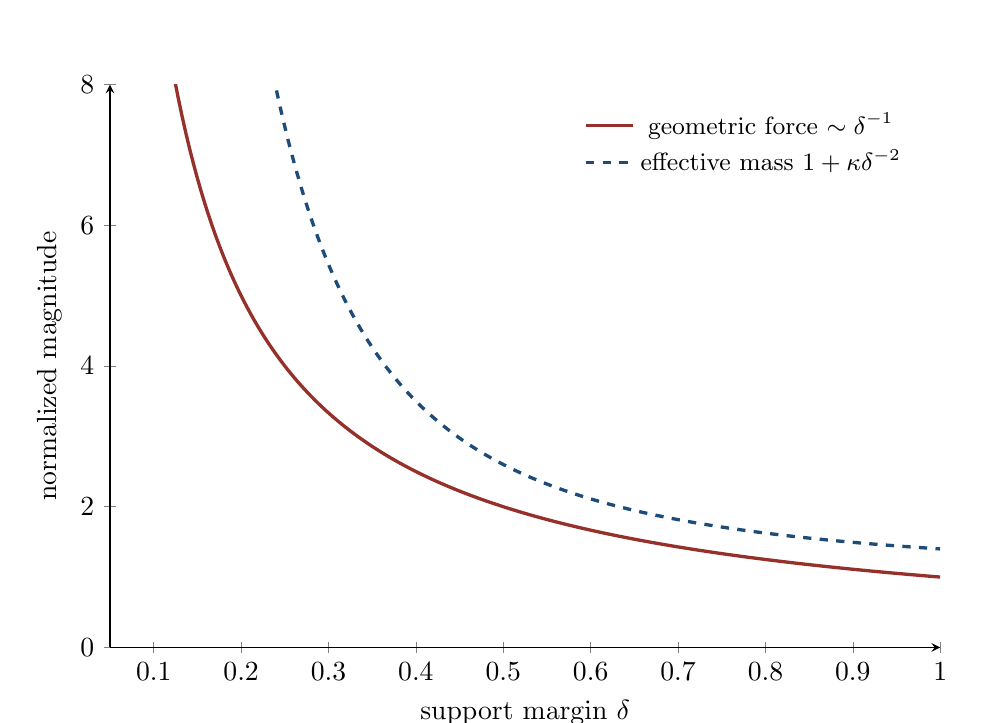
\begin{tikzpicture}
\begin{axis}[
 width=\linewidth,height=0.72\linewidth,
 axis lines=left,xlabel={support margin $\delta$},ylabel={normalized magnitude},
 xmin=0.05,xmax=1,ymin=0,ymax=8,
 samples=220,domain=0.05:1,
 legend style={draw=none,font=\small,at={(0.97,0.97)},anchor=north east}]
 \addplot[very thick,paperred] {1/x};
 \addlegendentry{geometric force $\sim\delta^{-1}$}
 \addplot[very thick,dashed,paperblue] {1+0.4/x^2};
 \addlegendentry{effective mass $1+\kappa\delta^{-2}$}
\end{axis}
\end{tikzpicture}
\caption{Competing singular scalings.}
\end{subfigure}\hfill
\begin{subfigure}[t]{0.48\linewidth}
\centering
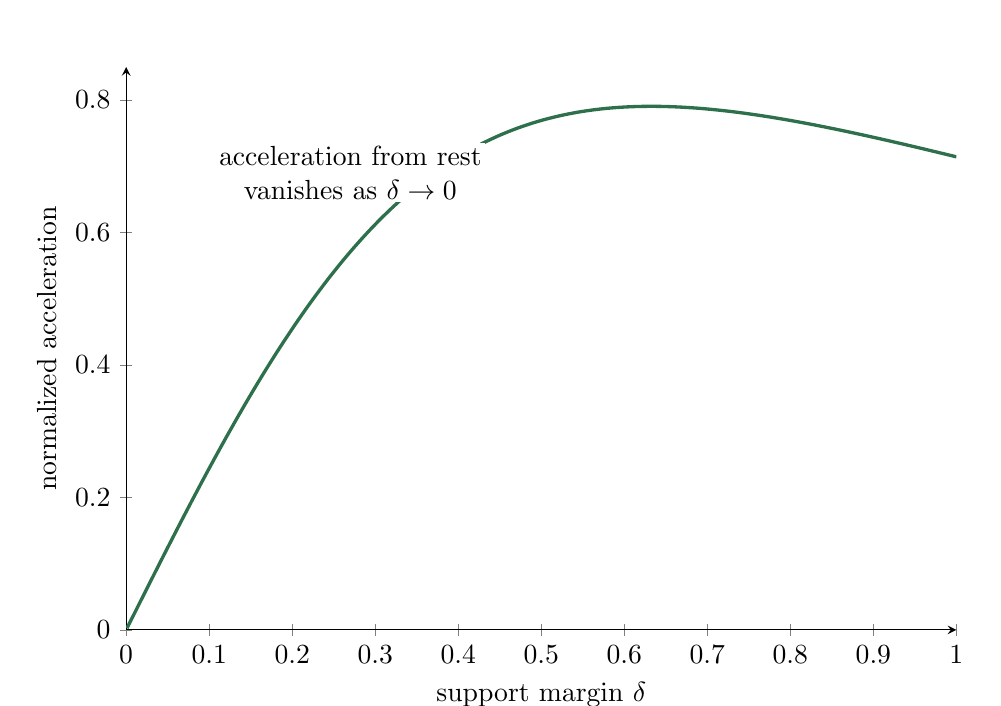
\begin{tikzpicture}
\begin{axis}[
 width=\linewidth,height=0.72\linewidth,
 axis lines=left,xlabel={support margin $\delta$},ylabel={normalized acceleration},
 xmin=0,xmax=1,ymin=0,ymax=0.85,
 samples=220,domain=0.001:1]
 \addplot[very thick,papergreen] {x/(0.4+x^2)};
 \node[align=center,fill=white,inner sep=1.2pt] at (axis cs:0.27,0.69) {acceleration from rest\\vanishes as $\delta\to0$};
\end{axis}
\end{tikzpicture}
\caption{Regularized rest acceleration.}
\end{subfigure}
\caption{The ideal geometric force grows near the support limit, but rotational inertia grows faster.  Curves show asymptotic forms with $\kappa=2/5$.}
\label{fig:regularization}
\end{figure}

\section{Dissipation and contact feasibility}

\subsection{Normal force}

Under quasi-static balance normal to the rail-center plane, equal rail forces satisfy
\begin{equation}
  2N\delta\approx mg\cos\beta,
  \qquad
  N\approx\frac{mg\cos\beta}{2\delta}.
  \label{eq:normalforce}
\end{equation}
Dynamic normal acceleration adds correction terms, but \cref{eq:normalforce} gives the principal geometric scaling.

A reduced rolling-resistance model is
\begin{equation}
  F_d
  =\mu_rmg\frac{\cos\beta}{\delta}\sgn(v)
   +c_1v+c_2|v|v,
  \label{eq:dissipation}
\end{equation}
where the first term is the sum of the resistance at the two rods.  A regularized odd function should replace $\sgn(v)$ in numerical work near $v=0$.

\subsection{No-slip feasibility}

Let $\bm F_{t,i}$ be the tangential contact force at rail $i$.  Sticking requires
\begin{equation}
  \|\bm F_{t,i}\|\leq\mu_sN_i,
  \label{eq:frictioncone}
\end{equation}
with transition to microslip or sliding when the inequality is saturated.  Monitoring normal force and static-friction demand is essential in rolling-ball systems \citep{Putkaradze2018}.  Because both the required spin and normal load become extreme near small $\delta$, terminal high-speed play is expected to encounter slip or material compliance before the rigid geometric limit.

It is useful to define admissibility guards
\begin{align}
  G_{\mathrm{geom}}&:=1-\eta,\\
  G_N&:=N_{\max}-N,\\
  G_\mu&:=\mu_sN-\|\bm F_t\|,\\
  G_\omega&:=\omega_{\max}-\frac{|v|}{R\delta}.
  \label{eq:rigidguards}
\end{align}
The intended two-contact rolling mode requires each guard to remain positive.

\section{Time-dependent opening, twist, and compound-pulse work}

The handle motion changes $\alpha(t)$, individual attitudes, and the axial angles $\phi_\pm(t)$.  The constraint manifold and material surfaces are therefore time dependent, allowing the player to exchange both translational and rotational energy with the ball.

Define the reduced mechanical energy
\begin{equation}
  E(x,v,\alpha)=\frac12M(x,\alpha)v^2+V(x,\alpha).
  \label{eq:energy}
\end{equation}

\begin{proposition}[Reduced energy identity]
Along solutions of \cref{eq:reducedmotion},
\begin{equation}
  \dot E
  =\left(V_\alpha-\frac12M_\alpha v^2\right)\dot\alpha
   -F_dv.
  \label{eq:energyidentity}
\end{equation}
\end{proposition}

\begin{proof}
Differentiate \cref{eq:energy}, substitute \cref{eq:reducedmotion}, and cancel the $M_xv^3/2$ terms.  Equivalently, use the standard identity $\dot E=-\partial\mathcal L/\partial t+Qv$ with $Q=-F_d$.
\end{proof}

For a scalar open--close pulse over $[t_0,t_1]$,
\begin{equation}
  \Delta E
  =\int_{t_0}^{t_1}
  \left(V_\alpha-\frac12M_\alpha v^2\right)\dot\alpha\,\dd t
  -\int_{t_0}^{t_1}F_dv\,\dd t.
  \label{eq:pulseenergy}
\end{equation}
The first integral can be nonzero even if $\alpha(t_1)=\alpha(t_0)$ because $x$ and $v$ change during the cycle.  A finite compound pulse may be parameterized as
\begin{equation}
  \bm u_p(t)
  =\begin{bmatrix}\alpha(t)&\phi_+(t)&\phi_-(t)\end{bmatrix}^{T}
  =\bm u_0+\bm A f\!\left(\frac{t-t_p}{\tau_p}\right),
  \label{eq:pulseform}
\end{equation}
where $\bm A$, $\tau_p$, and $t_p$ are the vector amplitude, duration, and center time.  The relative phases of opening, common twist, and differential twist determine whether energy is placed in longitudinal motion, axial ball spin, vertical constraint motion, or slip.

In the complete contact model, the instantaneous actuator power is
\begin{equation}
  P_{\mathrm{contact}}
  =\sum_i\bm F_i\cdot\bm v_{r,i}.
  \label{eq:contactpower}
\end{equation}
For axial twist alone, if $Q_i=\bm F_i\cdot\bm q_i$ is the circumferential tangential force,
\begin{equation}
  P_{\phi}=r\sum_i Q_i\dot\phi_i.
  \label{eq:twistpower}
\end{equation}
Equation \cref{eq:energyidentity} is the scalar-opening reduction of this general moving-contact work.  A physically observed ``pulse'' may therefore be a vector event in $(\alpha,\phi_+,\phi_-)$ rather than a purely open--close motion.

If a pulse supplies net useful energy $\Delta E_{\mathrm{use}}$ while $M$ varies little over the pulse, then
\begin{equation}
  v_+^2\approx v_-^2+\frac{2\Delta E_{\mathrm{use}}}{M}.
  \label{eq:pulsespeed}
\end{equation}
This equation formalizes the player's sensation of ``pulsing the ball.''

\section{Small rail compliance}

\subsection{Beam equation}

Let $w_i(s,t)$ be the outward transverse deflection of rod $i$, measured along rod coordinate $s\in[0,L]$.  Euler--Bernoulli theory gives
\begin{equation}
  \rho_bA_bw_{i,tt}+c_bw_{i,t}+EI_bw_{i,ssss}=q_i(s,t),
  \label{eq:beam}
\end{equation}
where $EI_b$ is flexural rigidity and $c_b$ is distributed damping \citep{Meirovitch2001}.  The lateral component of a localized contact load is approximately
\begin{equation}
  q_i(s,t)=N_i(t)\eta(t)\,\delta_D(s-x(t))+q_{h,i}(s,t).
  \label{eq:beamload}
\end{equation}
For a simply supported rod, the static compliance at the load point is
\begin{equation}
  C_b(x)=\frac{x^2(L-x)^2}{3EI_bL},
  \label{eq:beamcompliance}
\end{equation}
although the actual boundary conditions should be measured.


\subsection{Torsional elasticity and phase lag}

A rod that is rotated at the handle need not rotate as a perfectly rigid body.  Let $\vartheta_i(s,t)$ be elastic twist relative to the commanded axial angle $\phi_i(t)$.  Saint--Venant torsion gives
\begin{equation}
  \rho_bJ_p\vartheta_{i,tt}
  +c_t\vartheta_{i,t}
  -GJ_t\vartheta_{i,ss}
  =\tau_i(s,t),
  \label{eq:torsionpde}
\end{equation}
where $J_p$ is the polar area moment, $J_t$ the torsion constant, and $G$ the shear modulus.  For a circular rod, $J_t=J_p=\pi r^4/2$.  A circumferential contact force produces the localized torque
\begin{equation}
  \tau_i(s,t)
  \approx rQ_i(t)\delta_D(s-x(t))+\tau_{h,i}(s,t).
  \label{eq:torsionload}
\end{equation}
The local material angle entering \cref{eq:rodangularvelocity} is $\phi_i(t)+\vartheta_i(x(t),t)$.  Torsional compliance therefore introduces phase lag, stored energy, and oscillation into a nominal $5^\circ$ hand rotation.  At high pulse rates the contact surface may continue moving after the handle reverses.

\subsection{Static compliance closure}

Let $\eta_c=d_c/(2a)$ be the commanded rigid separation.  Each rail deflects outward by approximately $w=C_bN\eta$, so the total separation change is $2w$.  Using \cref{eq:normalforce},
\begin{equation}
  \eta
  =\eta_c+\Lambda\frac{\eta}{\delta},
  \qquad
  \Lambda:=\frac{C_bmg\cos\beta}{2a}.
  \label{eq:complianceimplicit}
\end{equation}
Equivalently,
\begin{equation}
  \eta_c(\eta)=\eta\left(1-\frac{\Lambda}{\delta}\right).
  \label{eq:complianceclosure}
\end{equation}

\begin{proposition}[Compliance-induced fold]
\label{prop:fold}
Assume $0<\Lambda<1$.  The quasi-static branch \cref{eq:complianceclosure} has a fold at
\begin{equation}
  \delta_*=\Lambda^{1/3},
  \qquad
  \eta_*=\sqrt{1-\Lambda^{2/3}},
  \qquad
  \eta_{c,*}=\left(1-\Lambda^{2/3}\right)^{3/2}.
  \label{eq:fold}
\end{equation}
Thus finite compliance terminates the monotone support branch before the rigid command value $\eta_c=1$.
\end{proposition}

\begin{proof}
Since $\dd(\eta/\delta)/\dd\eta=\delta^{-3}$,
\begin{equation}
  \frac{\dd\eta_c}{\dd\eta}=1-\frac{\Lambda}{\delta^3}.
\end{equation}
The fold occurs at $\delta^3=\Lambda$.  Substitution into $\eta^2+\delta^2=1$ and \cref{eq:complianceclosure} gives the remaining formulas.
\end{proof}

The first-order height perturbation caused by a small separation error $\Delta d$ is
\begin{equation}
  \Delta h\approx-\frac{d}{4h}\Delta d.
  \label{eq:heightamplification}
\end{equation}
Because $N=O(\delta^{-1})$ and $|h_d|=O(\delta^{-1})$, the formal composition of load-induced deflection and geometric height sensitivity scales as $O(\delta^{-2})$.  This explains why visually slight bending can dominate the terminal region.

\begin{figure}[t]
\centering
\begin{subfigure}[t]{0.49\linewidth}
\centering
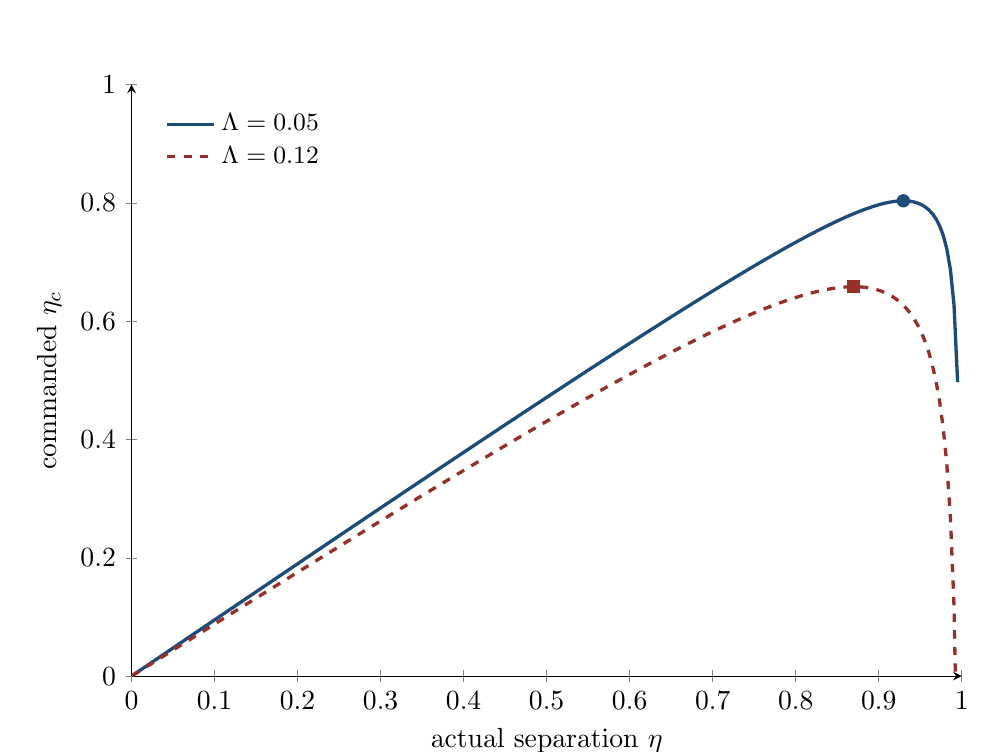
\begin{tikzpicture}
\begin{axis}[
 width=\linewidth,height=0.75\linewidth,
 axis lines=left,xlabel={actual separation $\eta$},ylabel={commanded $\eta_c$},
 xmin=0,xmax=1,ymin=0,ymax=1,
 samples=230,domain=0.001:0.995,
 legend style={draw=none,font=\small,at={(0.03,0.97)},anchor=north west}]
 \addplot[very thick,paperblue] {x*(1-0.05/sqrt(1-x^2))};
 \addlegendentry{$\Lambda=0.05$}
 \addplot[very thick,dashed,paperred] {x*(1-0.12/sqrt(1-x^2))};
 \addlegendentry{$\Lambda=0.12$}
 \addplot[only marks,mark=*,mark size=2.2pt,paperblue] coordinates {(0.9297,0.8035)};
 \addplot[only marks,mark=square*,mark size=2.2pt,paperred] coordinates {(0.8699,0.6583)};
\end{axis}
\end{tikzpicture}
\caption{Static branch and fold points.}
\label{fig:foldplot}
\end{subfigure}\hfill
\begin{subfigure}[t]{0.48\linewidth}
\centering
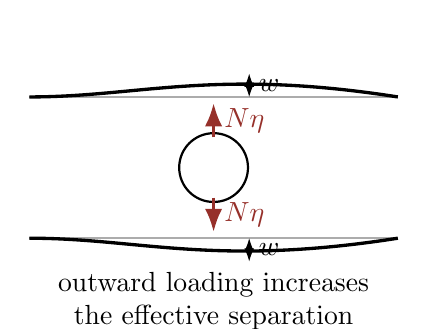
\begin{tikzpicture}[scale=0.78,>=Latex]
 \draw[thick,gray!65] (0,1.15) -- (6,1.15);
 \draw[thick,gray!65] (0,-1.15) -- (6,-1.15);
 \draw[very thick] (0,1.15) .. controls (1.8,1.15) and (3.0,1.62) .. (6,1.15);
 \draw[very thick] (0,-1.15) .. controls (1.8,-1.15) and (3.0,-1.62) .. (6,-1.15);
 \draw[fill=white,thick] (3,0) circle (0.56);
 \draw[->,very thick,paperred] (3,0.49) -- (3,1.05) node[midway,right] {$N\eta$};
 \draw[->,very thick,paperred] (3,-0.49) -- (3,-1.05) node[midway,right] {$N\eta$};
 \draw[<->] (3.58,1.15) -- (3.58,1.53) node[midway,right] {$w$};
 \draw[<->] (3.58,-1.15) -- (3.58,-1.53) node[midway,right] {$w$};
 \node[align=center] at (3,-2.18) {outward loading increases\\the effective separation};
\end{tikzpicture}
\caption{Symmetric lateral bending.}
\label{fig:bending}
\end{subfigure}
\caption{Compliance is not merely a small correction.  The reduced static closure develops a fold, providing a mechanism for premature release or snap-through.}
\label{fig:compliance}
\end{figure}

\section{Hybrid contact and terminal release}

The game does not remain in one smooth dynamical mode.  Let $g_i(q)$ be the normal gap at contact $i$ and $N_i$ the corresponding compressive normal force.  Unilateral contact is represented by
\begin{equation}
  g_i\geq0,
  \qquad N_i\geq0,
  \qquad g_iN_i=0.
  \label{eq:complementarity}
\end{equation}
Together with \cref{eq:frictioncone}, these relations define a nonsmooth mechanical system \citep{Brogliato2016}.  Relevant modes are:
\begin{enumerate}[label=\textnormal{M\arabic*:},leftmargin=3.2em]
  \item symmetric two-contact rolling;
  \item two-contact rolling with microslip;
  \item asymmetric or one-contact motion;
  \item free flight after release;
  \item impact with the target board or collection tray.
\end{enumerate}
During free flight,
\begin{equation}
  m\ddot{\bm r}_C=m\bm g+\bm F_{\mathrm{air}},
  \label{eq:freeflight}
\end{equation}
followed by an impact map or compliant impact law.  The full terminal event is therefore a transition from constrained rolling to ballistic motion, not merely a continuation of \cref{eq:reducedmotion}.

The compliance fold adds another guard,
\begin{equation}
  G_{\mathrm{fold}}:=\delta^3-\Lambda.
  \label{eq:foldguard}
\end{equation}
A conservative safe set can require
\begin{equation}
\begin{aligned}
  G_{\mathrm{geom}}&>0, &
  G_{\mathrm{fold}}&>0, &
  G_N&>0, &
  G_\mu&>0, &
  G_\omega&>0,\\
  G_{\phi,i}&:=\phi_{\max}-|\phi_i|>0,
  &G_{\Delta}&:=s_{\Delta,\max}-|s_\Delta|>0.
\end{aligned}
  \label{eq:guards}
\end{equation}

\begin{figure}[t]
\centering
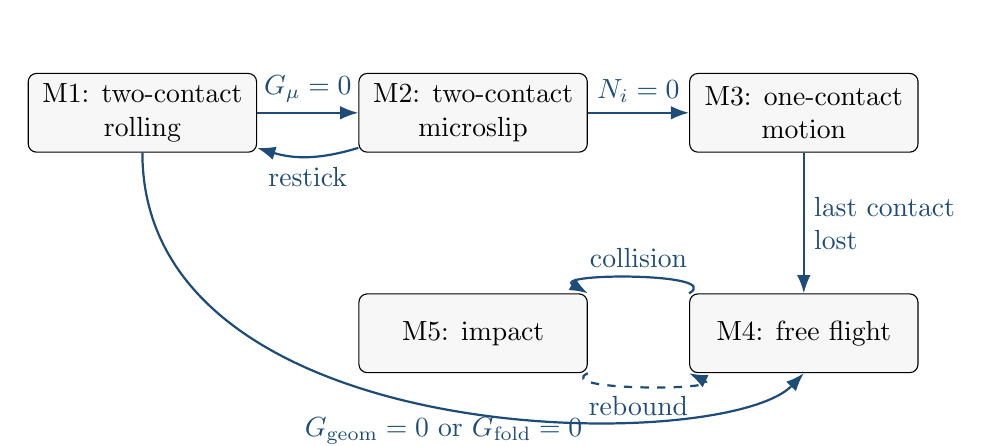
\begin{tikzpicture}[
  >=Latex,
  mode/.style={draw,rounded corners=3pt,minimum width=29mm,minimum height=10mm,align=center,fill=gray!6},
  event/.style={->,thick,paperblue}
]
  \node[mode] (roll) at (-4.2,1.25) {M1: two-contact\\rolling};
  \node[mode] (slip) at (0,1.25) {M2: two-contact\\microslip};
  \node[mode] (one) at (4.2,1.25) {M3: one-contact\\motion};
  \node[mode] (impact) at (0,-1.55) {M5: impact};
  \node[mode] (flight) at (4.2,-1.55) {M4: free flight};

  \draw[event] (roll) -- node[above] {$G_\mu=0$} (slip);
  \draw[event] (slip) to[bend left=17] node[below] {restick} (roll);
  \draw[event] (slip) -- node[above] {$N_i=0$} (one);
  \draw[event] (one) -- node[right,align=left] {last contact\\lost} (flight);
  \draw[event] (flight.north west) .. controls (3.20,-0.78) and (1.00,-0.78) ..
    node[above] {collision} (impact.north east);
  \draw[event,dashed] (impact.south east) .. controls (1.00,-2.28) and (3.20,-2.28) ..
    node[below] {rebound} (flight.south west);
  \draw[event] (roll.south) .. controls (-4.2,-3.10) and (3.2,-3.10) ..
    node[below,align=center] {$G_{\mathrm{geom}}=0$ or $G_{\mathrm{fold}}=0$} (flight.south);
\end{tikzpicture}
\caption{Hybrid mode graph.  The scoring release is a controlled guard crossing into free flight; an early or asymmetric crossing is a failure.}
\label{fig:hybrid}
\end{figure}

\section{Target-specific viability and speed risk}

\subsection{Recoverable states}

Let the state include rigid, actuator, and retained beam variables,
\begin{equation}
  z=(x,v,\alpha,\dot\alpha,
  \phi_c,\dot\phi_c,\phi_\Delta,\dot\phi_\Delta,
  q_b,\dot q_b,q_t,\dot q_t,\ldots).
  \label{eq:state}
\end{equation}
Let $\safe$ be the state set in which the desired contact mode and all actuator/contact guards are valid, and let $\target_k$ be the terminal set corresponding to scoring target $k$.

\begin{definition}[Target-specific viability kernel]
For horizon $T$, define
\begin{equation}
  \K_k(T)
  :=\left\{z_0\in\safe:\ \exists u(\cdot)\in\controls
  \text{ such that }z(t)\in\safe\text{ until }\target_k\text{ is reached}\right\}.
  \label{eq:viability}
\end{equation}
\end{definition}

This is a controlled viability/capture-basin problem in the sense of \citet{Aubin1991,SaintPierre1994}.  In a projection onto $(x,v)$, part of the boundary may be summarized by a target-specific critical curve $v_{\mathrm{crit},k}(x)$.  A high-performance path uses a small reserve
\begin{equation}
  \varepsilon(x)=v_{\mathrm{crit},k}(x)-v(x)>0.
  \label{eq:reserve}
\end{equation}
The curve is global: it represents remaining distance, available control, friction, compliance, and terminal timing, not merely a local detachment speed.

\begin{figure}[t]
\centering
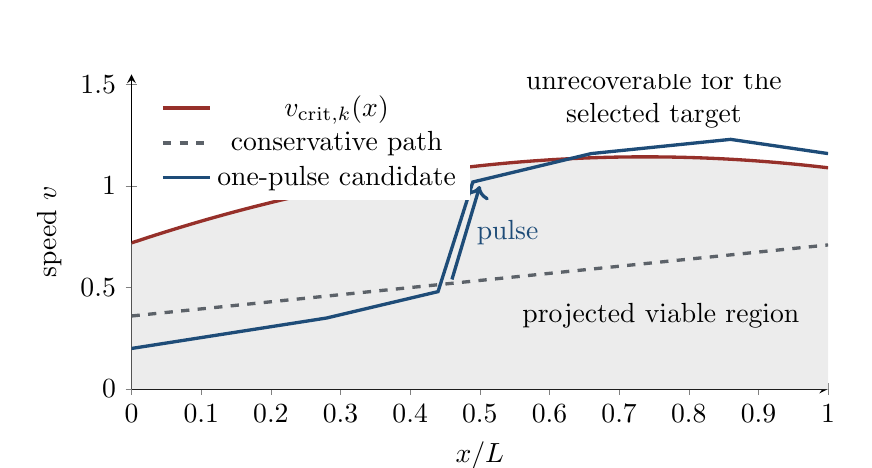
\begin{tikzpicture}
\begin{axis}[
 width=0.86\linewidth,height=0.46\linewidth,
 axis lines=left,xlabel={$x/L$},ylabel={speed $v$},
 xmin=0,xmax=1,ymin=0,ymax=1.55,
 samples=180,domain=0:1,
 legend style={draw=none,at={(0.03,0.97)},anchor=north west}]
 \addplot[name path=crit,very thick,paperred] {0.72+1.15*x-0.78*x^2};
 \addlegendentry{$v_{\mathrm{crit},k}(x)$}
 \addplot[name path=axis,draw=none,forget plot] {0};
 \addplot[gray!15,forget plot] fill between[of=crit and axis];
 \addplot[very thick,dashed,papergray] {0.36+0.35*x};
 \addlegendentry{conservative path}
 \addplot[very thick,paperblue] coordinates {(0,0.20) (0.28,0.35) (0.44,0.48) (0.49,1.02) (0.66,1.16) (0.86,1.23) (1.0,1.16)};
 \addlegendentry{one-pulse candidate}
 \draw[->,very thick,paperblue] (axis cs:0.46,0.54) -- (axis cs:0.50,1.00) node[midway,right] {pulse};
 \node[align=center] at (axis cs:0.76,0.36) {projected viable region};
 \node[align=center] at (axis cs:0.75,1.43) {unrecoverable for the\\selected target};
\end{axis}
\end{tikzpicture}
\caption{Schematic target-specific phase portrait.  Record-seeking play approaches the viability boundary from below, whereas reliability-oriented play retains a larger reserve.}
\label{fig:phaseportrait}
\end{figure}

\subsection{Release timing uncertainty}

Suppose the desired release position is centered in a longitudinal interval of width $\Delta x$.  Let residual position error and motor timing error be independent Gaussians,
\begin{equation}
  e_x\sim\mathcal N(0,\sigma_x^2),
  \qquad
  e_t\sim\mathcal N(0,\sigma_t^2).
\end{equation}
The linearized release-position error is $e=e_x+ve_t$, hence
\begin{equation}
  \sigma_{\mathrm{eff}}^2(v)=\sigma_x^2+v^2\sigma_t^2.
  \label{eq:sigmaeff}
\end{equation}
The probability of releasing inside the target window is
\begin{equation}
  p_{\mathrm{hit}}(v)
  =\Prob\{|e|\leq\Delta x/2\}
  =\erf\!\left(
  \frac{\Delta x}{2\sqrt2\sqrt{\sigma_x^2+v^2\sigma_t^2}}
  \right).
  \label{eq:phit}
\end{equation}

\begin{proposition}[Timing risk increases strictly with speed]
\label{prop:timing}
If $\sigma_t>0$ and $\Delta x>0$, then $p_{\mathrm{hit}}'(v)<0$ for every $v>0$.
\end{proposition}

\begin{proof}
The denominator in the argument of $\erf$ is strictly increasing for $v>0$, and $\erf$ is strictly increasing.  Their composition is therefore strictly decreasing.
\end{proof}

The elementary release-time window obeys
\begin{equation}
  \Delta t_{\mathrm{release}}\approx\frac{\Delta x}{v}.
  \label{eq:releasewindow}
\end{equation}
Thus speed can improve reach while unavoidably reducing release robustness.

\subsection{Score objectives}

Let $S(v)$ denote score conditional on an aggressiveness class and $P_s(v)$ its success probability.  Expected-score play maximizes
\begin{equation}
  J(v)=P_s(v)S(v).
\end{equation}
At an interior optimum,
\begin{equation}
  \frac{S'(v)}{S(v)}=-\frac{P_s'(v)}{P_s(v)}.
  \label{eq:scorebalance}
\end{equation}
The fractional gain in score is balanced by the fractional loss of reliability.

A record-seeking objective is different.  For target $k$ with per-attempt success probability $p_k$, the probability of at least one success in $n$ approximately independent attempts is
\begin{equation}
  P_{k,n}=1-(1-p_k)^n.
  \label{eq:multipleattempts}
\end{equation}
A player seeking the maximum target at least once can rationally accept lower per-attempt reliability.

\begin{figure}[t]
\centering
\begin{subfigure}[t]{0.49\linewidth}
\centering
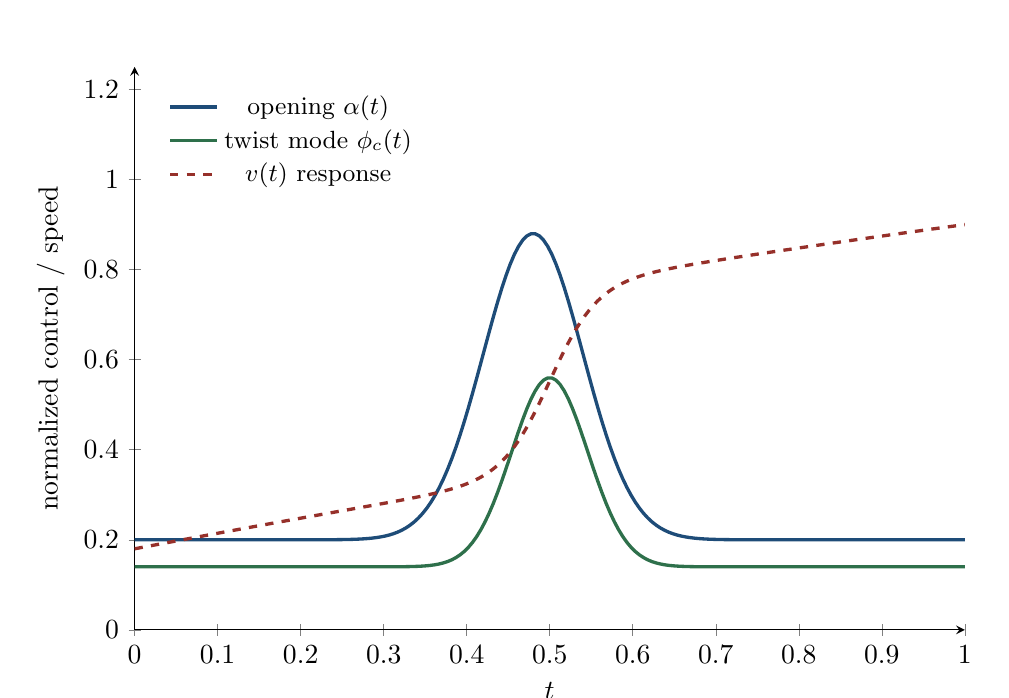
\begin{tikzpicture}
\begin{axis}[
 width=\linewidth,height=0.72\linewidth,
 axis lines=left,xlabel={$t$},ylabel={normalized control / speed},
 xmin=0,xmax=1,ymin=0,ymax=1.25,
 legend style={draw=none,font=\small,at={(0.03,0.97)},anchor=north west},
 samples=200,domain=0:1]
 \addplot[very thick,paperblue] {0.20+0.68*exp(-((x-0.48)/0.085)^2)};
 \addlegendentry{opening $\alpha(t)$}
 \addplot[very thick,papergreen] {0.14+0.42*exp(-((x-0.50)/0.065)^2)};
 \addlegendentry{twist mode $\phi_c(t)$}
 \addplot[very thick,dashed,paperred] {0.18+0.35*x+0.42/(1+exp(-35*(x-0.50)))-0.05*x^2};
 \addlegendentry{$v(t)$ response}
\end{axis}
\end{tikzpicture}
\caption{Compound opening--twist pulse and speed response.}
\end{subfigure}\hfill
\begin{subfigure}[t]{0.49\linewidth}
\centering
\begin{tikzpicture}
\begin{axis}[
 width=\linewidth,height=0.72\linewidth,
 axis lines=left,xlabel={speed $v$},ylabel={$p_{\mathrm{hit}}(v)$},
 xmin=0,xmax=3.2,ymin=0.55,ymax=1.02]
 \addplot[very thick,papergreen,smooth] coordinates {
 (0.0,0.9992) (0.2,0.9989) (0.4,0.9976) (0.6,0.9940)
 (0.8,0.9857) (1.0,0.9707) (1.2,0.9483) (1.4,0.9194)
 (1.6,0.8859) (1.8,0.8496) (2.0,0.8123) (2.2,0.7752)
 (2.4,0.7392) (2.6,0.7048) (2.8,0.6722) (3.0,0.6416)
 (3.2,0.6129)};
 \node[align=center] at (axis cs:2.25,0.93) {timing robustness\\falls with speed};
\end{axis}
\end{tikzpicture}
\caption{Evaluation of \cref{eq:phit}.}
\end{subfigure}
\caption{The same action that increases reach can move the trajectory toward the viability boundary and reduce terminal hit probability.  Curves are illustrative, not fitted to a particular machine.}
\label{fig:pulseandrisk}
\end{figure}

\section{Risk-sensitive optimal control}

A rate-limited reduced state can be written
\begin{equation}
  z=(x,v,\alpha,a,
  \phi_c,\Omega_c,\phi_\Delta,\Omega_\Delta,
  q_b,\dot q_b,q_t,\dot q_t),
  \qquad a=\dot\alpha,
  \label{eq:controlstate}
\end{equation}
with bounded opening jerk $j_\alpha$ and twist angular accelerations $u_c,u_\Delta$.  Retaining one bending mode and one torsional mode gives
\begin{align}
  \dot x&=v,\\
  M\dot v&=-V_x-\frac12M_xv^2-M_\alpha av-F_d+Q_b+F_\phi,\\
  \dot\alpha&=a,
  &\dot a&=j_\alpha,\\
  \dot\phi_c&=\Omega_c,
  &\dot\Omega_c&=u_c,\\
  \dot\phi_\Delta&=\Omega_\Delta,
  &\dot\Omega_\Delta&=u_\Delta,\\
  \ddot q_b+2\zeta_b\omega_b\dot q_b+\omega_b^2q_b&=B_bN\eta,\\
  \ddot q_t+2\zeta_t\omega_t\dot q_t+\omega_t^2q_t&=B_t rQ_\Delta.
  \label{eq:controlsystem}
\end{align}
Here $F_\phi$ is zero in the ideal local parallel circular limit but is generated by divergence, skew, noncircularity, or slip.  The system is subject to bounds on opening, individual axial angle, rates, torques, contact forces, and all hybrid guards.

A risk-sensitive objective is
\begin{equation}
  \max_{(j_\alpha,u_c,u_\Delta)(\cdot)}\left\{
  \E[S(X_{\mathrm{impact}})]
  -\lambda\Prob\{\text{failure}\}
  -\int_0^T
   \left(\gamma_\alpha j_\alpha^2+
   \gamma_cu_c^2+\gamma_\Delta u_\Delta^2\right)\dd t
  -\xi T
  \right\}.
  \label{eq:riskobjective}
\end{equation}
The weight $\lambda$ selects a point on the speed-risk frontier.

\begin{proposition}[Bang-bang tendency]
Suppose a reduced model is control-affine,
\begin{equation}
  \dot z=f(z)+g(z)u,
  \qquad u\in[u_{\min},u_{\max}],
  \label{eq:affine}
\end{equation}
with a minimum-time or terminal-payoff problem whose Pontryagin Hamiltonian is affine in $u$.  Away from singular arcs, an optimal control takes values only at $u_{\min}$ or $u_{\max}$ almost everywhere.
\end{proposition}

\begin{proof}
The Hamiltonian has the form
$H=\lambda_z^Tf(z)+\lambda_z^Tg(z)u+\ell(z)$.  For fixed state and costate it is affine in $u$, so its extremum over a compact interval occurs at an endpoint unless the switching function $\lambda_z^Tg(z)$ vanishes on an interval.  This is the standard maximum-principle argument \citep{Pontryagin1962}.
\end{proof}

This result explains why a short high-authority action is natural, but not how many switches are optimal.  A schematic pulse-location merit function is
\begin{equation}
  \mathcal Q(x_p)
  =B_{\mathrm{energy}}(x_p)
  -L_{\mathrm{remaining}}(x_p)
  -\lambda R_{\mathrm{terminal}}(x_p).
  \label{eq:pulsevalue}
\end{equation}
Early pulses leave more distance for dissipation and error growth.  Late pulses leave little useful travel and perturb the most sensitive region.  These competing effects make an interior $x_p^*$ plausible without implying $x_p^*=L/2$.

\begin{conjecture}[Single dominant compound-pulse regime]
\label{conj:onepulse}
There exists a nonempty parameter regime of rail slope, opening and twist authority, rolling loss, bending/torsional compliance, actuator rate limits, and terminal-risk weight in which the maximum-score optimal policy contains one dominant intermediate vector pulse in $(\alpha,\phi_+,\phi_-)$, followed by a high-speed arc lying just inside the target-specific viability boundary.
\end{conjecture}

The conjecture is deliberately conditional.  The dominant event may be mostly separation control, mostly common twist, or a phased combination including differential twist.  Strong dissipation, weak actuation, accurate high-bandwidth feedback, or a sharply varying viability boundary can favor several smaller pulses.  The decisive test is to solve the calibrated problem without constraining pulse count or control direction and determine whether one compound pulse emerges.

\section{Dimensionless groups and mechanical regimes}

Use the rail length $L$, gravitational speed $\sqrt{gL}$, and time $\sqrt{L/g}$ to define
\begin{equation}
  X=\frac{x}{L},
  \qquad
  U=\frac{v}{\sqrt{gL}},
  \qquad
  \tau=t\sqrt{\frac{g}{L}}.
\end{equation}
Important dimensionless groups are
\begin{align}
  \rho_r&=\frac rR,
  &\Pi_\alpha&=\frac{L\tan\alpha}{R+r},\\
  \Pi_b&=\frac{mgL^3}{EI_bR},
  &\Pi_c&=\frac{c_1}{M_0\sqrt{g/L}},\\
  \mathrm{St}_p&=\tau_p\sqrt{\frac gL},
  &\Lambda&=\frac{C_bmg\cos\beta}{2(R+r)},\\
  \Phi_{\max}&=\phi_{\max},
  &\Pi_{\dot\phi}&=\frac{r\dot\phi_{\max}}{\sqrt{gL}},\\
  \Pi_{\mathrm{tor}}&=\sqrt{\frac{\rho_bJ_p gL}{GJ_t}},
  &\epsilon_r&=\max_i|\epsilon_i|.
  \label{eq:dimensionlessgroups}
\end{align}
Together with $\mu_r$, $\mu_s$, $\beta$, independent rod-attitude limits, and actuator bounds, these parameters distinguish several regimes:
\begin{enumerate}[label=(\alph*),leftmargin=2.2em]
  \item \emph{geometry dominated}: large $\Pi_\alpha$, low loss, stiff rods;
  \item \emph{dissipation dominated}: rolling loss erases early pulse energy;
  \item \emph{compliance dominated}: $\Lambda$ is large enough that the fold precedes the desired release;
  \item \emph{twist dominated}: $\Pi_{\dot\phi}$ is large enough that rod-surface motion materially changes spin or propulsion;
  \item \emph{torsion dominated}: handle motion is phase-lagged by elastic twist;
  \item \emph{actuator limited}: finite opening/twist rate, torque, or jerk prevents impulsive control;
  \item \emph{risk dominated}: timing variance and narrow terminal geometry determine the optimum.
\end{enumerate}
The conjectured one-pulse strategy is expected only in a subset of this parameter space.

\section{System identification and falsification protocol}

A credible validation requires measurement of one physical apparatus rather than guessed parameters.  The following protocol identifies the hierarchy of models and tests \cref{conj:onepulse}.

\begin{enumerate}[leftmargin=2.25em]
  \item \textbf{Rigid geometry and attitude.} Measure $R$, $r$, $L$, the two centerlines $\bm c_i(s,u_i)$, $\beta_i$, $\gamma_i$, and the full separation map.  Compare side-view center height with \cref{eq:h,eq:zV}.
  \item \textbf{Axial rotation.} Instrument each rod with an angular marker or encoder, measure the actual range corresponding to the nominal $5^\circ$ bound, and identify common/differential handle modes.
  \item \textbf{Rolling kinematics.} Mark the ball and estimate all three spin components from high-speed video.  Test \cref{eq:reff,eq:twistinterpretation} in low-slip trials.
  \item \textbf{Dissipation.} Run coast-down experiments at several fixed openings to identify $\mu_r$, $c_1$, and $c_2$.
  \item \textbf{Bending and torsion.} Apply known transverse loads and handle torques to identify $C_b(x)$, bending modes, $GJ_t$, damping, and torsional phase lag.  Test the fold scaling in \cref{eq:fold} by changing ball mass or rod stiffness.
  \item \textbf{Circularity and surface anisotropy.} Measure runout/ovality and friction versus axial angle to determine whether the absolute $\phi_i$ affects geometry or only $\dot\phi_i$ affects surface velocity.
  \item \textbf{Compound-pulse work.} Record synchronized opening, $\phi_\pm$, ball position, speed, three-axis spin, bending, and torsion during controlled cycles.  Compare measured work with \cref{eq:pulseenergy,eq:twistpower}.
  \item \textbf{Hybrid guards.} Identify onset of slip, one-contact motion, and release as functions of $(x,v,\alpha,\dot\alpha)$.
  \item \textbf{Human strategies.} Compare smooth conservative, many-small-pulse, one-pulse, and unrestricted expert trials.
  \item \textbf{Unconstrained optimization.} Solve \cref{eq:controlsystem,eq:riskobjective} using direct collocation, dynamic programming, or stochastic model-predictive control without prescribing pulse count.
\end{enumerate}

The one-pulse conjecture gains support only if the independently calibrated optimizer repeatedly discovers a dominant intermediate pulse and predicts how its location changes after controlled perturbations to mass, friction, bending/torsional stiffness, axial-angle range, slope, or target geometry.  If the optimizer instead finds multiple pulses or a smooth singular arc, that outcome refutes the conjecture for the tested regime.

\section{Discussion}

\subsection{What the model establishes}

Several conclusions follow directly from the stated assumptions.

First, the geometry-induced drive is exact within the symmetric cross-sectional model: opening the rods lowers the ball center, and uphill acceleration begins when \cref{eq:criticalopening} is satisfied.

Second, the symmetric no-slip geometry has an exact local rolling radius $R\delta$.  This causes effective rotational inertia to grow as $\delta^{-2}$ and regularizes the apparent terminal force singularity at zero speed.  Independent axial rod rotation adds a second ball-spin component and a differential compatibility condition; these are absent from a one-input opening model.

Third, small compliance can have a non-small qualitative effect.  The static closure in \cref{eq:complianceclosure} develops a calculable fold before the rigid geometric limit.  This provides a concrete mechanism for early release, snap-through, and extreme sensitivity to rod stiffness.

Fourth, the speed-risk tradeoff is not merely verbal.  Under the release-error model, hit probability is strictly decreasing in speed.  High speed becomes rational only because the scoring geometry or reach constraint changes the payoff set.

\subsection{What remains conjectural}

The model does not prove that a particular commercial machine has a one-pulse optimum.  That conclusion depends on measured dissipation, independent opening/twist limits, circularity, bending and torsional compliance, terminal geometry, and the player's objective.  Nor does the reduced model replace the full three-dimensional contact equations near slip or release.  It provides a structured hierarchy:
\begin{equation}
  \text{rigid reduced model}
  \subset
  \text{compliant modal model}
  \subset
  \text{full nonsmooth contact model}.
\end{equation}
The simpler levels are useful only while validated against the next level and against experiment.

\subsection{Interpretation of maximum risk}

``Maximum risk'' should not mean arbitrary recklessness.  It means operation near the boundary of the target-specific viability kernel.  For a given target and uncertainty model, there is a largest useful aggressiveness at which the fractional score gain still compensates for the fractional loss of success probability.  A record-seeking player with many attempts chooses a different boundary reserve from a player maximizing average score per attempt.

\section{Conclusion}

The Space Force / Shoot-the-Moon mechanism is a compact example of controlled transport on a moving, compliant constraint manifold.  The support variable $\delta$ controls center height, contact orientation, rolling radius, normal load, and effective inertia.  Xu, Groff, and Burg supplied the foundational rigid nonholonomic dynamics and model-based position control.  The present extension shows that independent rod attitudes and approximately five-degree axial rotations add surface-velocity controls that govern ball axial spin, vertical compatibility, slip, and---outside the parallel circular limit---longitudinal propulsion and braking.  Rod opening creates geometry-induced uphill drive, while compound opening--twist motion exchanges energy with the ball.  Rolling resistance and traction constraints limit this mechanism.  Bending is amplified near release, torsion creates phase lag, and contact loss produces a hybrid transition to free flight.

For scoring, the relevant object is the target-specific viability kernel.  Maximum-performance trajectories approach its boundary; timing uncertainty makes terminal hit probability decrease strictly with speed.  This formalizes the observed paradox that the route to the maximum score can also be the route with the smallest robustness margin.  Bang-bang theory makes a short high-authority compound pulse mechanically plausible.  Whether the optimal strategy contains exactly one intermediate vector pulse in separation and rod twist is now a precise, falsifiable question for system identification and unconstrained optimal-control computation.

\appendix

\section{Full vector rolling equations}
\label{sec:vector}

Let $\bm r_C$ be the ball-center position, $\bm\omega$ its angular velocity, and $\bm\rho_i$ the vector from the center to contact $i$.  The sphere contact-point velocity is
\begin{equation}
  \bm v_{c,i}=\dot{\bm r}_C+\bm\omega\times\bm\rho_i.
\end{equation}
With centerline and angular motion given by \cref{eq:rodcenterline,eq:rodangularvelocity}, the rod material velocity is \cref{eq:rodsurfacevelocity}.  Ideal rolling requires
\begin{equation}
  \bm P_{T,i}(\bm v_{c,i}-\bm v_{r,i})=\bm 0,
  \qquad
  \bm P_{T,i}=\bm I-\bm n_i\bm n_i^T.
  \label{eq:vectorrolling}
\end{equation}
The Newton--Euler equations are
\begin{align}
  m\ddot{\bm r}_C
  &=m\bm g+\sum_i(N_i\bm n_i+\bm F_{t,i})+\bm F_{\mathrm{air}},\\
  \bm I_C\dot{\bm\omega}+\bm\omega\times(\bm I_C\bm\omega)
  &=\sum_i\bm\rho_i\times\bm F_{t,i}+\bm\tau_{\mathrm{ext}}.
  \label{eq:NewtonEuler}
\end{align}
Together with \cref{eq:complementarity,eq:frictioncone}, these form a differential-algebraic or complementarity system.  The scalar equation \cref{eq:reducedmotion} is its symmetric centerline reduction.

\section{Compact reduced model}

A minimal simulation model is
\begin{align}
  d&=d_0+2x\tan\alpha,
  &\eta&=\frac{d}{2(R+r)},
  &\delta&=\sqrt{1-\eta^2},\\
  V&=mg\left(x\sin\beta+(R+r)\delta\right),
  &M&=m\left(1+\frac{\kappa}{\delta^2}\right),\\
  M\dot v&=-V_x-\frac12M_xv^2-M_\alpha\dot\alpha v-F_d,
  &\dot x&=v,\\
  F_d&=\mu_rmg\frac{\cos\beta}{\delta}\sgn(v)+c_1v+c_2|v|v,\\
  \omega_x&=-\frac rR\dot\phi_c,
  &s_\Delta&=r\dot\phi_\Delta-\eta\dot z_B.
  \label{eq:compactmodel}
\end{align}
Add the bending and torsional equations \cref{eq:beam,eq:torsionpde} or modal reductions, monitor the guards in \cref{eq:guards}, and switch to \cref{eq:freeflight} at release.

\section{Notation summary}

\begin{longtable}{@{}p{0.18\linewidth}p{0.72\linewidth}@{}}
\toprule
Symbol & Meaning \\
\midrule
$R,r$ & ball radius and rod radius \\
$m,I$ & ball mass and central moment of inertia \\
$x,L$ & longitudinal position and rail length \\
$\alpha$ & half of the included rod opening angle in the symmetric reduction \\
$\gamma_i,\beta_i$ & signed yaw and pitch of rod $i$ \\
$\phi_i$ & axial material rotation of rod $i$; nominal bound about $5^\circ$ \\
$\phi_c,\phi_\Delta$ & common and differential axial twist modes \\
$\beta$ & mean uphill inclination of the rail-center plane \\
$d$ & center-to-center rod separation \\
$a=R+r$ & ball-center to rod-center distance at contact \\
$\eta=d/(2a)$ & normalized separation \\
$\delta=\sqrt{1-\eta^2}$ & dimensionless support margin \\
$h=a\delta$ & ball-center height above the rod-center plane \\
$M$ & geometry-dependent translational effective mass \\
$N_i,\bm F_{t,i}$ & normal and tangential contact forces \\
$w_i,q_b$ & rod bending deflection and retained bending mode \\
$\vartheta_i,q_t$ & elastic torsional twist and retained torsion mode \\
$s_\Delta$ & differential-twist slip residual \\
$\Lambda$ & dimensionless static compliance parameter \\
$\K_k(T)$ & target-$k$ viability kernel over horizon $T$ \\
$\varepsilon$ & speed reserve below a projected viability boundary \\
\bottomrule
\end{longtable}


\section*{Acknowledgment and attribution}

The author gratefully recognizes Peng Xu for the foundational thesis treatment of the Shoot-the-Moon kinematics, Lagrangian and Newtonian dynamics, nonholonomic structure, controllers, and automated experimental platform, together with Richard E. Groff and Timothy C. Burg for the associated conference and journal work.  The present paper is intended as a standalone extension of that foundation, not a replacement for it.

\begin{thebibliography}{99}

\bibitem[Xu et al.(2010)]{Xu2010}
P. Xu, R. E. Groff, and T. C. Burg.
\newblock The rigid body dynamics of Shoot-the-Moon game and model-based controller design.
\newblock In \emph{Proceedings of the 2010 American Control Conference}, pages 396--401, 2010.
\newblock doi:10.1109/ACC.2010.5530797.

\bibitem[Xu et al.(2012)]{Xu2012}
P. Xu, R. E. Groff, and T. C. Burg.
\newblock Dynamics and control of the Shoot-the-Moon tabletop game.
\newblock \emph{Journal of Dynamic Systems, Measurement, and Control}, 134(5):051006, 2012.
\newblock doi:10.1115/1.4006223.

\bibitem[Xu(2011)]{Xu2011}
P. Xu.
\newblock \emph{Dynamics and Control of the Shoot-the-Moon Tabletop Game}.
\newblock M.S. thesis, Clemson University, All Theses 1209, 2011.
\newblock \url{https://open.clemson.edu/all_theses/1209/}.

\bibitem[De Moerlooze et al.(2011)]{DeMoerlooze2011}
K. De Moerlooze, F. Al-Bender, and H. Van Brussel.
\newblock Modeling of the dynamic behavior of systems with rolling elements.
\newblock \emph{International Journal of Non-Linear Mechanics}, 46(1):222--233, 2011.
\newblock doi:10.1016/j.ijnonlinmec.2010.09.003.

\bibitem[Johnson(1985)]{Johnson1985}
K. L. Johnson.
\newblock \emph{Contact Mechanics}.
\newblock Cambridge University Press, 1985.

\bibitem[Kalker(1990)]{Kalker1990}
J. J. Kalker.
\newblock \emph{Three-Dimensional Elastic Bodies in Rolling Contact}.
\newblock Kluwer Academic Publishers, 1990.

\bibitem[Putkaradze and Rogers(2018)]{Putkaradze2018}
V. Putkaradze and S. Rogers.
\newblock On the normal force and static friction acting on a rolling ball actuated by internal point masses.
\newblock arXiv:1810.04010, 2018.

\bibitem[Brogliato(2016)]{Brogliato2016}
B. Brogliato.
\newblock \emph{Nonsmooth Mechanics: Models, Dynamics and Control}.
\newblock Springer, third edition, 2016.

\bibitem[Aubin(1991)]{Aubin1991}
J.-P. Aubin.
\newblock \emph{Viability Theory}.
\newblock Birkh\"auser, 1991.

\bibitem[Saint-Pierre(1994)]{SaintPierre1994}
P. Saint-Pierre.
\newblock Approximation of the viability kernel.
\newblock \emph{Applied Mathematics and Optimization}, 29:187--209, 1994.
\newblock doi:10.1007/BF01204182.

\bibitem[Pontryagin et al.(1962)]{Pontryagin1962}
L. S. Pontryagin, V. G. Boltyanskii, R. V. Gamkrelidze, and E. F. Mishchenko.
\newblock \emph{The Mathematical Theory of Optimal Processes}.
\newblock Interscience Publishers, 1962.

\bibitem[Meirovitch(2001)]{Meirovitch2001}
L. Meirovitch.
\newblock \emph{Fundamentals of Vibrations}.
\newblock McGraw-Hill, 2001.

\end{thebibliography}

\end{document}
